\documentclass[../qm.tex]{subfiles}
\begin{document}
\section{A Small Intro to Some Wacky Units}
Since in particle physics usually we deal with particular calculations, it's preferable to avoid using the SI system of units, and instead pass to what I like to call, the system of \emph{God given units}, where the most common fundamental constants are taken as unitary, i.e. $\hbar=c=1$.\\
With this choice is also common to write energy in terms of $\mathrm{eV}$, i.e., using $c=1$ and $E=\gamma mc^2$, we have that
\begin{equation*}
	\left[ E \right]=\left[ m \right]=\mathrm{eV}
\end{equation*}
Using the dispersion relation we also get
\begin{equation*}
	E=p^2+m^2\implies{}\left[ p \right]=\mathrm{eV}
\end{equation*}
Therefore mass, energy and momentum are all expressed in $\mathrm{eV}$. Using that $1\ \mathrm{J}=(1.602)^{-1}\times 10^{19}\ \mathrm{eV}$ we get the conversion value
\begin{equation}
	1\ \mathrm{kg}=5.6\times 10^{35}\ \mathrm{eV}
	\label{eq:kgtoevconv}
\end{equation}
In these units we have that the mass of the electron $m_e$ and the mass of the proton $m_p$ are
\begin{equation}
	\begin{aligned}
		m_e&=9.109\times 10^{-31}\ \mathrm{kg}=0.511\ \mathrm{MeV}\\
		m_p&=1.673\times 10^{-27}\ \mathrm{kg}=938.3\ \mathrm{MeV}
	\end{aligned}
	\label{eq:massemassprot}
\end{equation}
The second consequence of taking $\hbar=c=1$ is that time can also be expressed in terms of $\mathrm{eV}$. In fact since $\left[ \hbar \right]=Js$ in the SI system, and $\hbar=1$ in the GGS\footnote{God Given System}, we have
\begin{equation*}
	\hbar=1.055\times10^{-34}\ \mathrm{Js}=6.583\times 10^{-22}\ \mathrm{MeVs}
\end{equation*}
Therefore
\begin{equation}
	1\ \mathrm{s}=\frac{1}{\hbar}\ \mathrm{MeV^{-1}}=1.519\times10^{21}\ \mathrm{MeV^{-1}}
	\label{eq:sinvmev}
\end{equation}
Combining both $\hbar c$ we have $\left[ \hbar c \right]=MeV m$, therefore we can think of expressing distances with this unit. Multiplying the constants we get
\begin{equation*}
	\hbar c=197.35\times10^{-15}\ \mathrm{MeV m}=197.35\ \mathrm{MeV fm}
\end{equation*}
This implies that
\begin{equation}
	1\ \mathrm{fm}=5.608\ \mathrm{GeV^{-1}}
	\label{eq:fmtogev}
\end{equation}
In these units is also quick to see that
\begin{equation}
	\alpha=\frac{e^2}{4\pi\epsilon_0\hbar c}\frac{1}{137}
	\label{eq:alphaconst}
\end{equation}
\section{Cross Section}
Consider a beam of particles colliding with a target which is long $d$. The $N_p$ particles of the beam will react with the $N_t$ particles of the target $N_R$ times in some time $T$.\\
\begin{figure}[H]
	\centering
	\begin{tikzpicture}
		\draw[->] (-2,0.5) -- (0.5,0.5);
		\draw[->] (-2,0.25) -- (0.5,0.25);
		\draw[->] (-2,0) -- (0.5,0);
		\draw[->] (-2,-0.25) -- (0.5,-0.25);
		\draw[->] (-2,-0.5) -- (0.5,-0.5);
		\draw[draw=black,pattern=north east lines] (1.5,-1) rectangle (2.2,1);
		\draw[->] (2.5,0) -- (3.5,0);
		\draw[->] (2.5,0.5) -- (3.5,1);
		\draw[->] (2.5,-0.5) -- (3.5,-1);
		\draw[<->] (1.5,-1.2) -- (2.2,-1.2);
		\node[below] at (1.85,-1.2) {$d$};
		\node[above] at (1.85,1) {\small Target};
		\node[below] at (-0.75,-0.5) {$N_p$};
		\node at (1.85,0) [rectangle,fill=white] (Nt) {\tiny$N_t$};
	\end{tikzpicture}
	\caption{Stylization of a beam of particles colliding with a target thick $d$}
	\label{fig:scatteringex}
\end{figure}
Considering the previous data, we can immediately say that the probabilty of interaction between a beam particle and a target particle in a time $T$, if the particle density of the target is $n_t$, is
\begin{equation}
	\sigma=\frac{1}{n_td}\frac{N_R/T}{N_p/T}\approx\frac{1}{n_td}\frac{\dot{N}_R}{\dot{N}_p}%\frac{1}{n_td}\frac{N_R}{N_p}
	\label{eq:csfirst}
\end{equation}
This probability is commonly known as the \emph{cross-section} for the reaction.\vfill\newpage
Consider now a beam with cross sectional surface $S$\\
\begin{minipage}{0.5\linewidth}
	\begin{figure}[H]
		\centering
		\begin{tikzpicture}
			\draw[fill=white!75!black] (-1.5,-1.5) rectangle (1.5,1.5);
			\fill[pattern=dots] (-1.5,-1.5) rectangle (1.5,1.5);
			\draw[fill=white] (0,0) circle (0.7);
			\draw[pattern=dots] (0,0) circle (0.7);
			\node at (-1.175,-1.205) [rectangle,fill=white!75!black] (St) {$S_t$};
			\node at (-1.01,1.205) [rectangle,fill=white!75!black] (nt) {\tiny$n_t$};
			\node at (0,0) [circle,fill=white] (S) {$S$};
		\end{tikzpicture}
		\caption{Cross section of the beam with surface $S$ hitting a target with surface $S_t$ and particle density $n_t$}
		\label{fig:csbeamscatter}
	\end{figure}
\end{minipage}
\begin{minipage}{0.45\linewidth}
	Since we have $S<S_t$ as in figure \eqref{fig:csbeamscatter} we have that the target is going to get hit in a fraction of his surface. Considering that the target is long $d$, we have that the amount of particles that might get hit by the beam will be
	\begin{equation}
		N_t=n_tSd\ \implies\ n_td=\frac{N_t}{S}
		\label{eq:ntbeamcs}
	\end{equation}
\end{minipage}\\
Inserting it back into the formula of the cross section we have
\begin{equation}
	\sigma=\frac{\dot{N}_R}{N_t}\frac{1}{S\dot{N}_p}
	\label{eq:sigmatottarpar}
\end{equation}
Since $S\dot{N}_p$ gives the amount of particles passing through a cross-sectional surface of the beam per unit time (i.e., a flux), we can define the flux of particles $\phi_p$ as follows
\begin{equation}
	\phi_p=S\derivative{N_p}{t}
	\label{eq:particlefluxscat}
\end{equation}
I.e.
\begin{equation}
	\sigma=\frac{1}{N_t\phi_p}\derivative{N_R}{t}
	\label{eq:sigmafluxscat}
\end{equation}
Noting also that if the particle beam is long $L$, if its particle density is $n_p$ we have, if $N_p$ is the total number of beam particles moving with average velocity $v_p$
\begin{equation*}
	N_p=n_pv_pS\dd t
\end{equation*}
And therefore, since $N_p$ is fixed
\begin{equation*}
	\phi_p=\frac{1}{S}\dv{N_p}{t}=n_pv_p
\end{equation*}
Which gives
\begin{equation*}
	\sigma=\frac{1}{n_pv_pN_t}\dv{N_R}{t}
\end{equation*}
And solving for $\dot{N}_R$ we have
\begin{equation}
	\dv{N_R}{t}=\sigma n_td\dv{N_p}{t}
	\label{eq:reactionperunittimescat}
\end{equation}
Which is the differential equation that gives the number of reactions per unit time. Note how $[\sigma]=L^2$, therefore it has units of $m^2$ in the S.I., in particle physics these units are quite uncomfortable since the cross sections evaluated are infinitesimally small, and another unit is used, the \emph{barn}. As follows there are the conversions
\begin{equation}
	1\ \mathrm{b}=10^{-28}\ \mathrm{m^2}
	\label{eq:barndef}
\end{equation}
For common reactions we have
\begin{equation}
	\begin{aligned}
		\mathrm{p+p\to X}&\qquad\sigma_{pp}\approx10\ \mathrm{mb}=10^{-30}\ \mathrm{m^2}\\
		\mathrm{\nu_e+p\to X}&\qquad\sigma_{\nu p}\approx10\ \mathrm{fb}=10^{-14}\ \mathrm{b}\\
		\mathrm{\chi+p\to X}&\qquad\sigma_{\chi p}\approx10^{-2}\ \mathrm{fb}=10^{-17}\ \mathrm{b}=10^{-45}\ \mathrm{m^2}
	\end{aligned}
	\label{eq:commonreaccscs}
\end{equation}
\subsection{Crossed Beam Interaction and Luminosity}
Consider two beams colliding frontally like they'd do in the LHC, a 27km particle accelerator ring.\\
%\begin{minipage}{0.5\linewidth}
\begin{figure}[H]
	\centering
	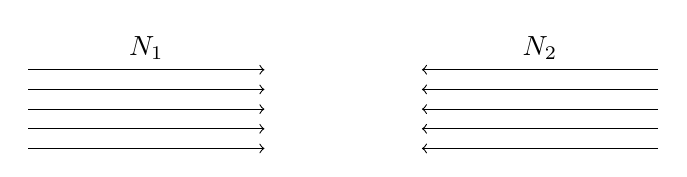
\begin{tikzpicture}
		\draw[->] (-4,0) -- (-1,0);
		\draw[->] (4,0) -- (1,0);
		\draw[->] (-4,0.5) -- (-1,0.5);
		\draw[->] (4,0.5) -- (1,0.5);
		\draw[->] (-4,0.25) -- (-1,0.25);
		\draw[->] (4,0.25) -- (1,0.25);
		\draw[->] (-4,-0.5) -- (-1,-0.5);
		\draw[->] (4,-0.5) -- (1,-0.5);
		\draw[->] (-4,-0.25) -- (-1,-0.25);
		\draw[->] (4,-0.25) -- (1,-0.25);
		\node[above] at (-2.5,0.5) {$N_1$};
		\node[above] at (2.5,0.5) {$N_2$};
	\end{tikzpicture}
	\caption{Schematization of the two beams colliding at some point inside a particle collider}
	\label{fig:twobeamcoll}
\end{figure}
The target we're now considering is a second beam with cross sectional surface $S_2=S_1=S$ and $N_2$ particles. Rewriting the formulas using $N_p=N_1$ and $N_t=N_2$ we get
\begin{equation*}
	\dv{N_R}{t}=\sigma n_2d\dv{N_1}{t}=\frac{\sigma}{S}N_2\dv{N_1}{t}
\end{equation*}
Using $\phi_1=S^{-1}\dot{N_1}$ we simply get
\begin{equation}
	\dv{N_R}{t}=\sigma\phi_1N_2
	\label{eq:crossbeamsigma}
\end{equation}
We can define a new quantity, $f_{int}$, i.e. the \emph{interaction frequency} of the beam, we have that the flux can be redefined as follows
\begin{equation}
	\phi_1=\frac{N_1f_{int}}{S}
	\label{eq:fluxfreq}
\end{equation}
And this gives
\begin{equation}
	\dv{N_R}{t}=\sigma\frac{N_1N_2 f_{int}}{S}=\sigma\mathcal{L}
	\label{eq:instlum}
\end{equation}
The new quantity $\mathcal{L}$ is called the \emph{instantaneous luminosity} of the collider and it has units of $\mathrm{L^{-2}T^{-1}}$ and is commonly expressed therefore in $\mathrm{Hz\ b^{-1}}$ or $\mathrm{Hz\ cm^{-2}}$.\\
Integrating the previous formula we get the \emph{integrated luminosity} $L$, measured in $\mathrm{b^{-1}}$
\begin{equation*}
	L=\int_{t_0}^{t_1}\mathcal{L}\dd t
\end{equation*}
\subsection{Higgs Bosons, Exclusive and Inclusive Cross Sections}
Going back to what we said for the luminosity of a detector, for the well known Large Hadron Collider we have
\begin{equation*}
	\mathcal{L}_{LHC}\approx10^{34}\ \mathrm{\frac{Hz}{cm^{2}}}=100\ \mathrm{\frac{Hz}{b}}
\end{equation*}
More specifically, during the years and the various runs it varied. The highest value was reached with run 3 of the LHC in 2018, where
\begin{equation*}
	L_{LHC}=163\ \mathrm{fb^{-1}}
\end{equation*}
This value can be used to estimate the number of events happened for a certain reaction. Take as an example the creation of Higgs boson
\begin{equation*}
	p+p\to H+X
\end{equation*}
The number of Higgs produced will be given using the integrated luminosity of LHC in run 3 and the cross section for the creation of $H+X$ particles
\begin{equation*}
	N_H=L\sigma_{HX}
\end{equation*}
Here $\sigma_{HX}\approx10^{-10}$ b and $\sqrt{s}=13$ TeV.
\begin{equation*}
	N_H=163\cdot10^{-10}\mathrm{b fb^{-1}}=163\cdot10^5
\end{equation*}
Therefore, in run 3, between 2015 and 2018 around 16 million Higgs bosons were produced in the LHC.\\
It's important tho to note that there are various ways a Higgs boson can decay, which will be what is going to be measured at the detector. These decays will be
\begin{equation*}
	\begin{aligned}
		H&\to bb\\
		H&\to\gamma\gamma\\
		H&\to ZZ\\
		H&\to WW
	\end{aligned}
\end{equation*}
The probability for having one of these decays is known as the \emph{branching factor} $BF$.\\
Suppose that now we want to see how many reactions of the kind $H\to\gamma\gamma$ happened in run 3, then we will have to weigh the total number of Higgs bosons with its branching factor
\begin{equation}
	N_{\gamma\gamma}=N_HBF_{H\to\gamma\gamma}
	\label{eq:htogammagamma}
\end{equation}
Suppose instead that we want to analyze a more complex decay of the Higgs boson
\begin{equation}
	\begin{aligned}
		H&\to ZZ\\
		ZZ&\to\left\{ \begin{aligned}
			&e^++e^-\\
			&\mu^++\mu^-\\
			&\tau^++\tau^-
	\end{aligned}\right.
	\end{aligned}
	\label{eq:HZZ}
\end{equation}
The branching factor for the $H\to ZZ$ is $BF_{H\to ZZ}=3\%$, which means that
\begin{equation*}
	N_{ZZ}=163\cdot10^5\cdot3\cdot10^{-2}=489\cdot10^{3}
\end{equation*}
This is not enough to check how many Higgs have been produced, since only the $Z+Z\to e^++e^-$ reaction is measured, and the total chain reaction we gotta consider becomes
\begin{figure}[H]
	\centering
	\begin{tikzpicture}
		\draw[->,color=sapienza] (-4,0) -- (-3.5,0) node[right] {$H+X$};
		\node[left,color=sapienza] at (-4,0) {$p+p$};
		\draw[->,color=sapienza] (-3.2,-0.2) -- (-3.2,-0.5) -- (-2.5,-0.5) node[right] {$Z^\pm+Z^\pm$};
		\draw[->,color=sapienza] (-2.25,-0.7) -- (-2.25,-1.5) -- (-1.7,-1.5) node[right] {$e^++e^-$};
		\draw[->,color=sapienza] (-1.2,-0.7) -- (-1.2,-1) -- (-0.7,-1) node[right] {$e^++e^-$};
	\end{tikzpicture}
\end{figure}
Therefore, the real number of measured Higgs bosons $N^\star_H$ will be
\begin{equation*}
	N_H^\star=\sigma_H LBF_{ZZ}BF_{Zee}^2=163\cdot10^5\cdot9\cdot10^{-4}\approx432
\end{equation*}
I.e., if the LHC's CMS detector was a perfect detector we would have measured \textit{at most} 432 Higgs bosons in the 4 full years of the third run.\\
A major problem now comes into play. What if I don't know the cross section for the reaction $\sigma_{HX}$?. In general we have that the number of particles is given by the number of counts of the detector, the integrated luminosity is measured directly, and the branching factors can be either measured or determined theoretically. Therefore, simply inverting and adding a factor $\varepsilon$ determining the efficiency of the detector, which accounts for imperfections in its surface, we have
\begin{equation*}
	\sigma_{HX}=\frac{N_H}{LBF_{HZZ}BF_{Zee}^2}\frac{1}{\varepsilon}
\end{equation*}
This is not enough for a proper determination of values, since in the LHC there are various reactions that get measured. We have that for each reaction with cross section $\sigma_i$, the total cross section of the $p+p\to X$ reaction is
\begin{equation}
	\sigma_{ppX}=\sum_{i=1}^n\sigma_i
	\label{eq:exccs}
\end{equation}
The cross sections on the right are known as \emph{exclusive cross sections} and the one on the left is the \emph{total cross section} for the measured event.\\
Note that in searching for the Higgs boson, we actually want to measure the photons from pair annihilation of the two electrons of the previous reaction, since their energies will peak around $m_Hc^2$, giving the complete reaction
\begin{figure}[H]
	\centering
	\begin{tikzpicture}
		\draw[->,color=sapienza] (-4,0) -- (-3.5,0) node[right] {$H+X$};
		\node[left,color=sapienza] at (-4,0) {$p+p$};
		\draw[->,color=sapienza] (-3.2,-0.2) -- (-3.2,-0.5) -- (-2.5,-0.5) node[right] {$Z^\pm+Z^\pm$};
		\draw[->,color=sapienza] (-2.25,-0.7) -- (-2.25,-1.5) -- (-1.7,-1.5) node[right] {$e^++e^-$};
		\draw[->,color=sapienza] (-1.2,-0.7) -- (-1.2,-1) -- (-0.7,-1) node[right] {$e^++e^-$};
		\draw[->,color=sapienza] (-0.2,-1.5) -- (0.2,-1.5) node[right] {$\gamma+\gamma$};
		\draw[->,color=sapienza] (0.8,-1) -- (1.2,-1) node[right] {$\gamma+\gamma$};
	\end{tikzpicture}
\end{figure}
Generally we're seeing the decay of a state $\ket{pp}$ into a state $\ket{e^+e^-e^+e^-}$, passing through a $Z^\pm$ state. Using SR we have
\begin{equation}
	\begin{aligned}
		P^\mu_{Z_1}&=p^\mu_{e^+_1}+p^\mu_{e^-_1}\\
		P^\mu_{Z_2}&=p^\mu_{e^+_2}+p^\mu_{e^-_2}
	\end{aligned}
	\label{eq:4momzz}
\end{equation}
The 4 moment of the 4 electrons is measured, and using the well known formula for the invariant mass we have that
\begin{equation*}
	m_{ZZ}=\sqrt{P^\mu_{(1)}P_\mu^{(2)}}
\end{equation*}
Which, also gives the energies of the emitted photons in the center of mass of the decay.\\
Measuring various combinations of such at LHC in 2012, finally a peak in counts of reactions at around $E^\star_{\gamma\gamma}\approx125$ GeV was measured, which corresponds to the measured mass of this famous boson.
\subsection{Mean Free Path}
Starting again for the usual and now well known relation for giving the number of reactions per unit time for some beam of particles hitting a target long $l$, we can imagine to generalize everything to differential lengths $l\to\dd x$, giving us
\begin{equation*}
	\dv{N_R}{t}=\sigma n_t\dv{N_p}{t}\dd x
\end{equation*}
The interaction probability will be
\begin{equation*}
	P_{int}=\frac{\dot{N}_R}{\dot{N}_p}=\sigma n_t\dd x= \sigma\frac{N_t}{S}
\end{equation*}
Define now an \emph{absorption coefficient} $\mu$. This coefficient indicates the amount of particles of the beam that get ``absorbed'' by the target per unit length. Using some reasoning with the previous formulae we must have that it must depend linearly to the linear density of particles of the target $n_t$, and therefore
\begin{equation}
	\mu=\sigma n_t
	\label{eq:absorptioncoeff}
\end{equation}
We have now that the pdf for the interaction energy is
\begin{equation}
	P_{int}=\mu\dd x
	\label{eq:interactionprob}
\end{equation}
This, must also be proportional to the derivative of the flux, since the flux must lower by some quantity while passing through the target. Finally we have
\begin{equation}
	\dv{\phi_p}{x}=-P_{int}\phi_p=-\mu\phi_p\dd x
	\label{eq:fluxdecrease}
\end{equation}
Solving the ODE we get
\begin{equation}
	\phi_p(x)=\phi_0e^{-\mu x}
	\label{eq:fluxred}
\end{equation}
Noting that $\mu$ has units of $L^{-1}$ we can imagine to define a length $\lambda$ as the inverse of this attenuation factor, known as the \emph{mean free path} of the particle.\\
The main utility of this length is that it can be used to determine the interaction cross section experimentally. In fact, imagine sending a flux of particles through $N$ targets with increasing lengths $d_i$ as in the next figure
\begin{figure}[H]
	\centering
	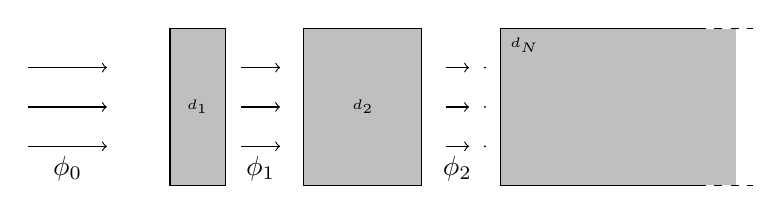
\begin{tikzpicture}
		\draw[->] (-5,-0.5) -- (-4,-0.5);
		\draw[->] (-5,0.5) -- (-4,0.5);
		\draw[->] (-5,0) -- (-4,0);
		\node[below] at (-4.5,-0.5) {$\phi_0$};
		\draw[fill=white!75!black] (-3.2,-1) rectangle (-2.5,1);
		\node at (-2.85,0) [rectangle,fill=white!75!black] (d1) {\tiny$d_1$};
		\draw[->] (-2.3,-0.5) -- (-1.8,-0.5);
		\draw[->] (-2.3,0) -- (-1.8,0);
		\draw[->] (-2.3,0.5) -- (-1.8,0.5);
		\node[below] at (-2.05,-0.5) {$\phi_1$};
		\draw[fill=white!75!black] (-1.5,-1) rectangle (0,1);
		\node at (-0.75,0) [rectangle,fill=white!75!black] (d2) {\tiny$d_2$};
		\draw[->] (0.3,-0.5) -- (0.6,-0.5);
		\draw[->] (0.3,0) -- (0.6,0);
		\draw[->] (0.3,0.5) -- (0.6,0.5);
		\node[below] at (0.45,-0.5) {$\phi_2$};
		\draw[fill=white!75!black,draw=white] (1,-1) rectangle (4,1);
		\draw (1,-1) -- (1,1);
		\draw (1,-1) -- (3.5,-1);
		\draw (1,1) -- (3.5,1);
		\draw[dashed] (3.5,-1) -- (4.2,-1);
		\draw[dashed] (3.5,1) -- (4.2,1);
		\node[below right] at (1,1) [rectangle,fill=white!75!black] (dn) {\tiny$d_N$};
		\draw (0.8,0.5) circle (0.1pt);
		\draw (0.8,0) circle (0.1pt);
		\draw (0.8,-0.5) circle (0.1pt);
	\end{tikzpicture}
	\caption{Example sketch of the experiment}
	\label{fig:sigmaexpermnt}
\end{figure}
Since $\phi\propto e^{-\mu x}$ we could use an exponential fit to find $\mu$. Using $\mu=\sigma n_t$ it's possible to estimate $\sigma$ if the properties of the target element are known
\section{Differential Cross Section}
Consider now a realistic approach for the collision of a beam of particles with a target. In this realistic approach the detectors will occupy part of the space around the target, and therefore there will be some preferred angles in order to detect properly the particle.\\
This final angle depends on the flight angle of the scattered particle.
\begin{figure}[H]
	\centering
	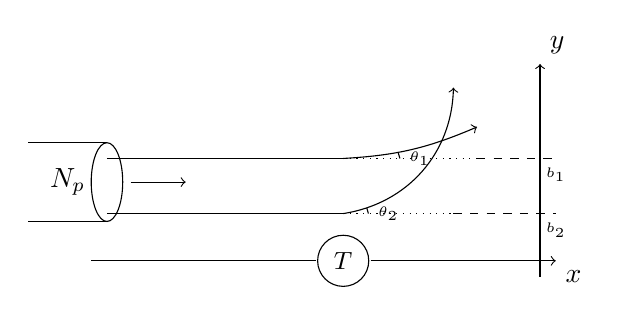
\begin{tikzpicture}
		\draw (-4,0.5) -- (-3,0.5);
		\draw (-4,-0.5) -- (-3,-0.5);
		\node at (-3.5,0) {$N_p$};
		\draw[->] (-2.7,0) -- (-2,0);
		\draw (-3,0) ellipse (0.2 and 0.5);
		\node at (0,-1) [circle,draw=black] (t) {\small$T$};
		\draw (-3.2,-1) -- (-0.35,-1);
		\draw[->] (0.35,-1) -- (2.7,-1) node[below right] {$x$};
		\draw[->] (2.5,-1.2) -- (2.5,1.5) node[above right] {$y$};
		\draw (-3,0.3) -- (0,0.3);
		\draw[dotted] (0,0.3) -- (1.7,0.3);
		\draw[dashed] (1.7,0.3) -- (2.7,0.3) node[below] {\tiny$b_1$};
		\draw[->] (0,0.3) to [bend right=10] (1.7,0.7);
		\draw (-3,-0.4) -- (0,-0.4);
		\draw[dotted] (0,-0.4) -- (1.4,-0.4);
		\draw[dashed] (1.4,-0.4) -- (2.7,-0.4) node[below] {\tiny$b_2$};
		\draw[->] (0,-0.4) to [bend right=40] (1.4,1.2);
		\draw[thin] (0.3,-0.33) to [bend left=10] (0.32,-0.4) node[right] {\tiny$\theta_2$};
		\draw[thin] (0.7,0.37) to [bend left=5] (0.72,0.3) node[right] {\tiny$\theta_1$};
	\end{tikzpicture}
	\caption{Sketch of the scattering process in study}
	\label{fig:diffcsscat}
\end{figure}
In the previous figure it's possible to see the sketch of this kind of scattering. The two parameters $b_1,b_2$ are known as the \emph{impact parameters} of the two particles, while the two angles $\theta_1,\theta_2$ are the \emph{flight angles} of the two particles.\\
In general, it's not hard to believe that this flight angle will depend on the impact parameter $b$ which is the vertical distance between the target and the unperturbed particle path's $y$ height.\\
From this supposition we can immediately say
\begin{equation*}
	\left\{ \begin{aligned}
			g(b)&=\theta\\
			f(\theta)&=b
	\end{aligned}\right.\implies\dd b\propto\dd\theta
\end{equation*}
Imagining a toroidal detector around the target we can transform this reasoning into 3D, where $\dd\theta\to\dd\Omega=\sin\theta\dd\theta\dd\varphi$. In this case, noting that $b\dd b=\sin\theta\dd\theta$ we get a new \emph{differential cross-section} $\dd\sigma$
\begin{equation}
	\dd\sigma=b\dd b\dd\theta
	\label{eq:ddcs}
\end{equation}
Manipulating this a bit we get
\begin{equation*}
	\dd\sigma=\dv{\sigma}{\Omega}\dd\Omega=\dv{\sigma}{\Omega}\abs{\sin\theta\dd\theta\dd\varphi}=b\dd b\dd\varphi
\end{equation*}
Or, rearranging everything
\begin{equation}
	\dv{\sigma}{\Omega}=\frac{b}{\abs{\sin\theta}}\abs{\dv{b}{\theta}}
	\label{eq:ddsigmaode}
\end{equation}
Where the absolute value comes from $\sigma>0$.
\begin{eg}[An Easy Example of Differential Cross-Section]
	As an example it's really exemplar finding the differential cross section for a particle hitting a rigid sphere with radius $R$.\\
	\begin{figure}[H]
		\centering
		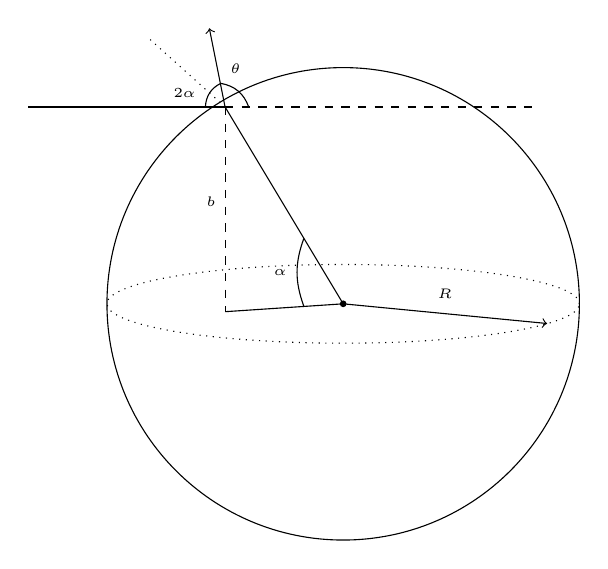
\begin{tikzpicture}
			\draw (0,0) circle (3cm);
			\draw[fill=black] (0,0) circle (1pt);
			\draw[dotted] (0,0) ellipse (3cm and 0.5cm);
			\draw[->] (0,0) -- (2.59,-0.25);
			\node at (1.29,0.125) (r) {\tiny$R$};
			\draw (-4,2.5) -- (-1.5,2.5);
			\draw[dashed] (-1.5,2.5) -- (2.5,2.5);
			\draw[->] (-1.5,2.5) -- (-1.7,3.5);
			\draw[thin] (-1.2,2.5) to [bend right=30] (-1.555,2.8) node[above right] (fa) {\tiny$\theta$};
			\draw[thin] (-1.555,2.8) to [bend right=30] (-1.75,2.5) node[above left] (2a) {\tiny$2\alpha$};
			\draw[dotted] (-1.5,2.5) --  (-2.5,3.4);
			\draw (0,0) -- (-1.5,2.5);
			\draw[dashed] (-1.5,2.5) -- (-1.5,-0.1);
			\node[left] at (-1.5,1.3) (b) {\tiny$b$};
			\draw (-0.5,-0.03) to [bend left=20] (-0.5,0.83);
			\node at (-0.8,0.4) (ang) {\tiny$\alpha$};
			\draw (-1.5,-0.1) -- (0,0);
		\end{tikzpicture}
		\caption{Quick sketch of the particle beam colliding with the cited sphere}
		\label{fig:diffcsspherescatter}
	\end{figure}
This rigid sphere can  be imagined as a potential wall in 3D spherical coordinates, where, simply
\begin{equation*}
	\pot(R)=\begin{dcases}
		0&r>R\\
		\infty&r<R
	\end{dcases}
\end{equation*}
It's obvious from the picture also that:
\begin{equation*}
	\left\{ \begin{aligned}
		b&=R\sin\alpha\\
		2\alpha+\theta&=\pi
	\end{aligned}\right.
\end{equation*}
Solving the second equations for $\alpha(\theta)$ we get that
\begin{equation*}
	\alpha=\frac{\pi-\theta}{2}
\end{equation*}
And therefore
\begin{equation*}
	\sin\left(\alpha\right)=\cos\left( \frac{\theta}{2} \right)\implies b=R\cos\left( \frac{\theta}{2} \right)
\end{equation*}
Deriving $b$ with respect to $\theta$ and getting its absolute value we get
\begin{equation*}
	\abs{\dv{b}{\theta}}=\frac{R}{2}\abs{\sin\left( \frac{\theta}{2} \right)}
\end{equation*}
And, simply substituting everything into \eqref{eq:ddsigmaode} we get
\begin{equation*}
	\dv{\sigma}{\Omega}=\frac{R^2}{2\abs{\sin\theta}}\cos\left( \frac{\theta}{2} \right)\sin\left( \frac{\theta}{2} \right)=\frac{R^2}{4}
\end{equation*}
Having now a simple differential equation for $\sigma$ we have finally
\begin{equation*}
	\sigma=\frac{R^2}{4}\int_{4\pi}^{}\dd\Omega=\pi R^2
\end{equation*}
Which means that, if the beam has cross sectional surface $S$, the probability of interaction of the beam with the sphere is
\begin{equation*}
	P_{int}=\frac{\pi R^2}{S}
\end{equation*}
This is in complete accord with the impulsive idea that the interaction probability in this case will be given from the exposed surface of the sphere divided by the surface of the beam, giving without problems a function of reactions in terms of cross-sectional surface of the beam
\begin{equation*}
	N_R(S)=\frac{\sigma}{S}=\frac{\pi R^2}{S}
\end{equation*}
\end{eg}
Having said all of this one might rightfully ask how would someone measure the differential cross section.\\
Start with hitting the target in question with a beam of particles with known flux, then the number of counts per unit time will be the usual well known formula
\begin{equation*}
	\dv{N_R}{t}=\sigma n_td\dv{N_p}{t}
\end{equation*}
Substituting inside this the differential quantities we have
\begin{equation*}
	\dv{N_R}{t}=n_td\dv{\sigma}{\Omega}\dv{N_p}{t}\dd\Omega
\end{equation*}
Expressing $n_td$ in terms of differential surface we can say immediately that
\begin{equation*}
	\frac{n_t}{S}\dv{N_p}{t}\dd S=\phi_p(x)N_t
\end{equation*}
Which gives
\begin{equation*}
	\dv{N_R}{t}=\phi_p(x)N_t\dv{\sigma}{\Omega}\dd\Omega
\end{equation*}
Since every term on the right is known and the number of counts per unit time is measured by the detector we can solve for the differential cross section, getting
\begin{equation}
	\dv{\sigma}{\Omega}=\frac{1}{\phi_p(x)N_t}\dv{N_R}{t}\frac{1}{\dd\Omega}
	\label{eq:measuredddcs}
\end{equation}
\end{document}
